\documentclass[12pt,a4paper]{report}
\usepackage{graphicx}
\usepackage{ctex}
\usepackage{indentfirst}
\graphicspath{{chapter/}{figures/}}
\usepackage{CJK}
\begin{document}


\chapter{研究背景及意义}
高降压比DC/DC变换器在工业、汽车、电信领域得到广泛应用。随着数据中心和云计算的不断发展,对电能传输的效率等指标提出了更高要求。在数据中心领域,流行的降压比为60V/48V/24V到5V/3.3V/1.8V。


Buck电路是一种典型的DC/DC拓扑结构。Buck电路结构简单,实现成本低,在电力电子与工业领域应用广泛。但是,对于一个二级Buck电路,要提高降压比,需要MOS管承受窄导通时间带来的大电流,这就在材料上对功率开关提出了极高要求。同时,高降压比所需要的极低占空比需要更高效的PWM,实际实施困难。这些因素限制了二级Buck电路的应用。


串联电容Buck电路(Series-capacitor Buck,SC-Buck)把开关电容和多相Buck结合到一起,形成一种新的Buck电路的拓扑结构。与传统的Buck电路相比,SC-Buck规模更小,效率更高,具有电流自平衡功能。如图1-1所示,两个电感交错放置于电路中,消除输出电容$C_o$上的电流纹波,同时还能分别减小两个电感的尺寸。图1-2表明,分到每条支路上的电压只有输入电压的一半。


实现高降压比的另一个趋势是使用磁性元件。实现方法有带倍流整流的全桥变换器(full-bridge converter with current-doubler rectifier),LLC,Sigma变换器和分接电感Buck变换器(tapped inductor Buck converter)等。在轻载时,全桥变换器无法实现所有主开关管的零电压开关(Zero-voltage Switching),导致轻载时转换效率下降,而且输出端的大电感会影响功率密度。在谐振频率下,LLC具有较高效率,但是系统不在谐振频率时的动态效率很低。为了解决这个问题,提出了将LLC和Buck结合的Sigma变换器。LLC负责谐振频率下的高效功率传输,Buck变换器负责瞬态响应。但是,由于LLC变换器在稳态时处理大部分的功率,Buck变换器在过渡时处理大部分的功率,因此LLC变换器和Buck变换器都必须设计成能够处理整个系统的功率。如此的并行结构将增大控制的复杂度。


Tapped inductor Buck转换器最初用于处理高降压比功率转换电路。然而,交错电感的漏感与开关电容产生共振,产生额外的电压环。基于混合变压器的Buck变换器(Hybrid-transformer-based Buck,HTB)增加了一个开关(S3)和一个电感,以获得软开关操作和较低的电压环,如图1-3所示。利用交错电感的漏感作为谐振电感,交错串联电容Buck(Series-capacitor tapped Buck,SC-TaB)变换器如图1-4所示。SC-TaB中的开关管$S_3$可以直接连接负载,也可以直接接地,另一种SC-TaB电路如图1-5所示。后者的两相交错配置的电路图如图1-6所示。开关管接地可以让控制更为简单。


SC-TaB和2ph-SC的主要优点是实现了所有开关管的ZVS,提高了转换效率。然而,随着降压比的增大,耦合电感的匝数比也随之增大,高匝数比会给耦合电感带来更多的应力,影响转换效率。为了克服这一缺点,并考虑到SC-Buck具有倍增降压比的能力,通过引入电容$C_1$,提出了一种新的变换器拓扑,如图1-7所示。新拓扑结构被称为交错串联电容分接Buck变换器(ISC-TaB)。该转换器将SC-Buck和SC-TaB的优点结合到一起。与传统的SC-TaB相比,它的降压比提高了一倍,使得该变换器更适合用于高降压比场合。
\begin{figure}[h]
    \centering
    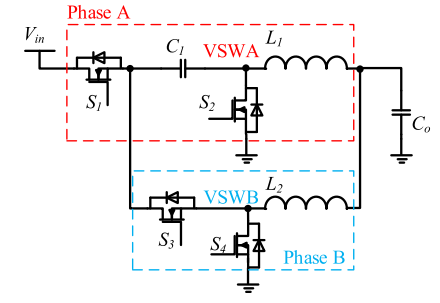
\includegraphics[width = 0.8\textwidth]{figures/SC-Buck.png}
    \caption{SC-Buck}
\end{figure}
\begin{figure}[h]
    \centering
    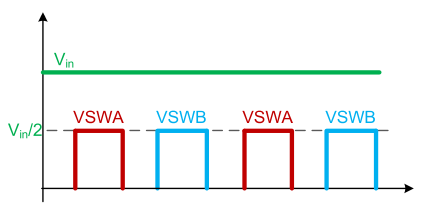
\includegraphics[width = 0.8\textwidth]{figures/SC-Buck_v.png}
    \caption{SC-Buck波形图}
\end{figure}
\begin{figure}[h]
    \centering
    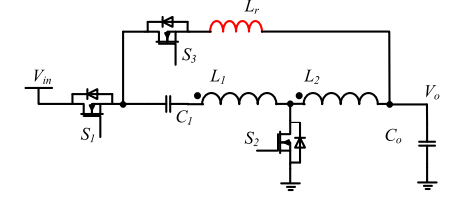
\includegraphics[width = 0.8\textwidth]{figures/HTB-Buck.png}
    \caption{HTB-Buck}
\end{figure}
\begin{figure}[h]
    \centering
    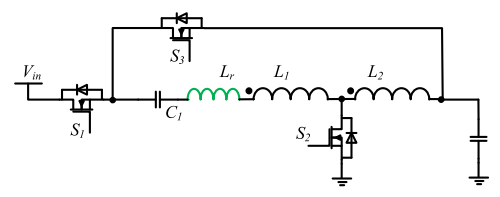
\includegraphics[width = 0.8\textwidth]{figures/SC-TaB1.png}
    \caption{SC-TaB,$S_3$接入负载}
\end{figure}
\begin{figure}[h]
    \centering
    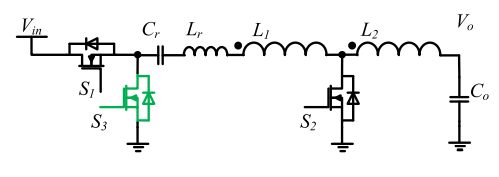
\includegraphics[width = 0.8\textwidth]{figures/SC-TaB.png}
    \caption{SC-TaB,$S_3$接地}
\end{figure}
\begin{figure}[h]
    \centering
    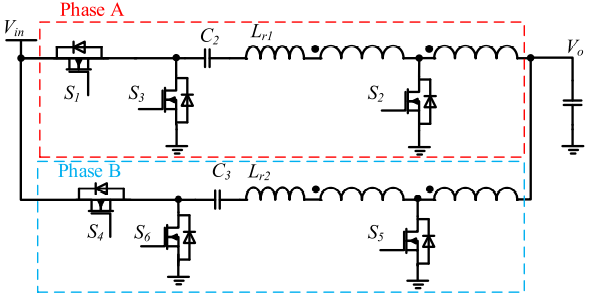
\includegraphics[width = 0.8\textwidth]{figures/2ph SC-TaB.png}
    \caption{2ph SC-TaB}
\end{figure}
\begin{figure}[h]
    \centering
    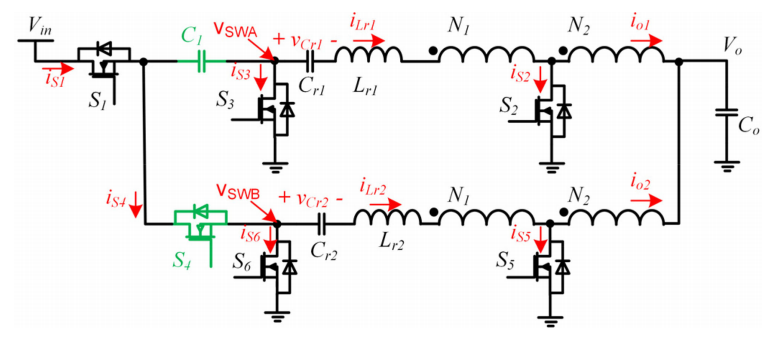
\includegraphics[width = 0.8\textwidth]{figures/circuit diagram1.png}
    \caption{ISC-TaB}
\end{figure}
\chapter{电路分析}
\section{电路结构}
\begin{figure}[h]
    \centering
    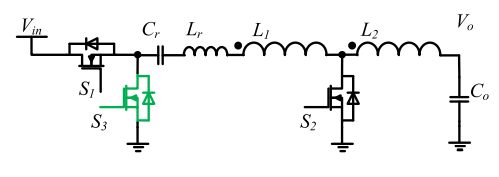
\includegraphics[width = 0.8\textwidth]{figures/SC-TaB.png}
    \caption{SC-TaB}
\end{figure}
\begin{figure}[h]
    \centering
    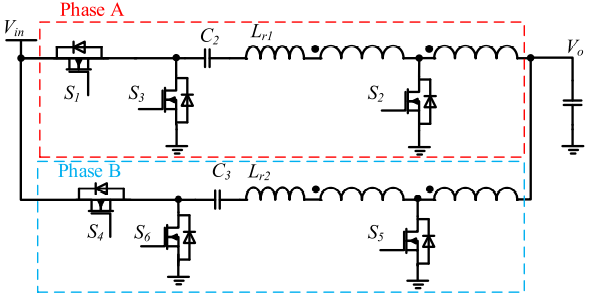
\includegraphics[width = 0.8\textwidth]{figures/2ph SC-TaB.png}
    \caption{2ph SC-TaB}
\end{figure}
\begin{figure}[h]
    \centering
    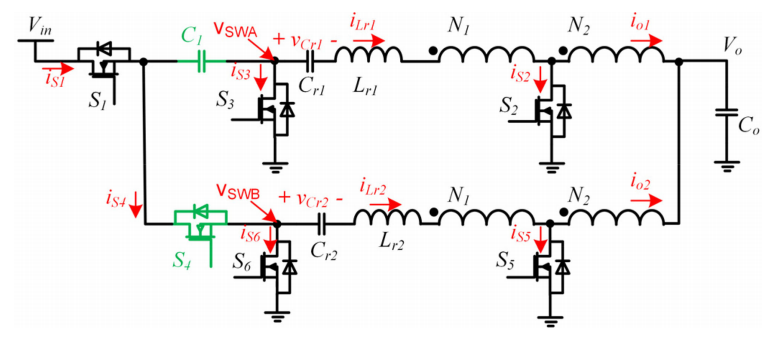
\includegraphics[width = 0.8\textwidth]{figures/circuit diagram1.png}
    \caption{ISC-TaB}
\end{figure}
\begin{figure}[h]
    \centering
    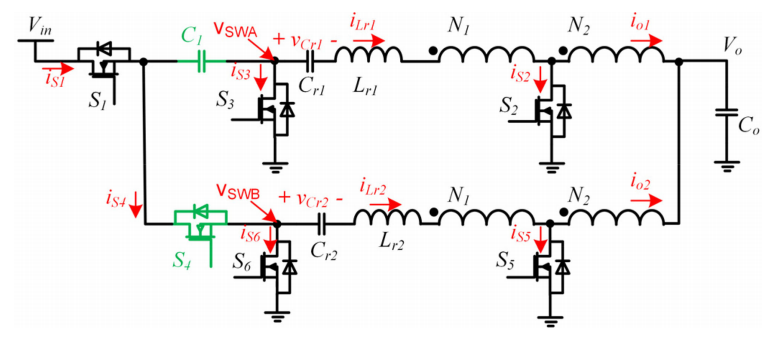
\includegraphics[width = 0.8\textwidth]{figures/circuit diagram1.png}
    \caption{ISC-TaB}
\end{figure}
电路采用了六个开关管,电容$C_1$将电路的两相分离。

\chapter{分析}
\section{电压转换率}
为了简化分析,使用$V_{cr2}$来表示开关周期内$C_{r2}$上的平均电压。
$T_s$是开关周期,$DT_s$表示从t0到t3的时间。
根据(1),在$[t0,t3]$期间,$L_{r2}$两端的平均电压为:

\begin{equation}
    V_{\mathrm{Lr} 2}=\frac{\frac{V_{\mathrm{in}}}{2}-V_{o}-V_{\mathrm{Cr} 2}}{1+\frac{L_{m}}{L_{r 2}} \cdot \frac{(n+1)^{2}}{n^{2}}}
\end{equation}

根据图7所示的电流关系,$L_m$上的电压在$[t0,t3]$期间为:

\begin{equation}
    V_{\mathrm{Lm}}=\frac{L_{m}}{L_{r 2}} \cdot\left(1+\frac{1}{n}\right) \cdot V_{\mathrm{Lr} 2}
\end{equation}

考虑到公式1和公式2,$L_{r2}$上的伏秒平衡关系为:

\begin{equation}
    V_{\mathrm{Lr} 2} \cdot D+\left(-V_{\mathrm{Cr} 2}+n V_{o}\right) \cdot(1-D)=0
\end{equation}

$L_{m}$上的伏秒平衡关系也可写为为:

\begin{equation}
    V_{\mathrm{Lm}} \cdot D+(1-D)\left(-n V_{o}\right)=0
\end{equation}

考虑公式(3)到(6),并假设$L_{r 1}=L_{r 2}=L_{r}$,则ISC-TaB电路的电压转换比为:

\begin{equation}
    \frac{V_{o}}{V_{\mathrm{in}}}=\frac{D}{2 \cdot\left(n+1+\frac{L_{r}}{L_{m}} \cdot \frac{n^{2}}{n+1}\right)}
\end{equation}

Buck,SC-Buck,SC-TaB和ISC-TaB的电压转换关系图已经绘制在图9中。如(7)和图9所示,
建议的ISC-TaB转换器的转换比为SC-TaB的一半。 如前所述,当前提出的的ISC-TaB是一种适用于高降压DC/DC应用的拓扑。

\section{波形推到}

S1和S4的电流波形可以基于电压转换器的输入给出。 $iS4$的派生变形将在本节中以示例的方式给出。 $P_{in}$代表当前变压器的总输入功率。 $I_{S4-avg}$则是 $I_{S4}$的平均值:

\begin{equation}
    I_{S4_{avg}} = \frac{P_{in}/2}{V_{in}/2}
\end{equation}

为了获得$i_{S4}$的最小值,$L_{r2}$的电流在$[t0,t3]$假设是线性的。那么$i_{S4}$的最小值可由以下关系推导

\begin{equation}
    i_{S4_{min}} =I_{S4_{avg}}-\frac{D T_{s}}{2} \cdot \frac{V_{\mathrm{Lr} 2}}{L_{r}}
\end{equation}

\end{document}

